\section{Historical: Broad OptShrink Comparisons: Full Numerical Record}

Study A tunes OptShrink on the original 2,048 validation observations and masks. Study B inherits that lookup and selects rank from each new block of observations. Neither study retrains the compact estimator. Each has two independent test banks, 126 primary cells and two separate stress cells. All 30 pilots are reused for the final fit, without additional observations. The inference lookup uses supplied noise and reference strength, not true channel power or path count.

Study A uses test-bank seeds 202610210001 and 202610310001; Study B uses 202610610001 and 202610710001. Each cell adds 100 times its zero-based index to the bank seed. Both use 16 worlds per cell and bank. The selected-model seeds are 9101, 9102 and 9103. Sources, settings and checkpoints are hashed before test generation. Settings remain frozen after the test data are inspected.

The primary score averages 126 per-cell dB ratio-of-sums NMSE values, after pooling the two equal-sized test banks within each cell. It is not the dB of one pooled error ratio. Learned scores average the three separate model scores. Bootstrap resampling preserves pairing within each bank/cell; confidence intervals condition on these weights and the offline validation choices. They do not cover repeated training or offline selection uncertainty.

\subsection{Declared Contrasts and All Comparators}

The numerical tables separate the declared average-dB contrasts, alternative error summaries, individual models, test banks and stress cases. These summaries are not interchangeable: a gain in one average does not establish a gain in every cell or at every error threshold. All individual-cell scores are retained in the evidence records.

\begin{table*}[!t]
\caption{Learned gain (positive favors learning), three-contrast-adjusted 95\% intervals within each study, and largest observed primary-cell deterioration. Cellwise safety is not established.}
\label{tab:broad-ci}\centering\footnotesize
\setlength{\tabcolsep}{4pt}
\begin{tabular}{@{}llrrr@{}}\toprule
Study & Comparator & Gain (dB) & Adjusted interval & Worst harm (dB)\\
\midrule
A & Offline OptShrink, selected placement & 0.537 & [0.450, 0.695] & 3.117\\
A & Offline OptShrink, in-loop & 0.565 & [0.477, 0.723] & 3.117\\
A & Offline OptShrink, final-only & 0.738 & [0.621, 0.925] & 3.686\\
B & Online rank + placement selection & -0.449 & [-0.569, -0.358] & 4.478\\
B & Online rank, in-loop & -0.507 & [-0.562, -0.437] & 5.495\\
B & Online rank, final-only & -0.076 & [-0.226, 0.025] & 3.445\\
\bottomrule
\end{tabular}
\end{table*}


\begin{table}[!t]
\caption{Study A: all primary averages and mean end-to-end CPU time. Fixed-budget labels denote EM updates, not matched runtime.}
\label{tab:all-A}\centering\footnotesize
\setlength{\tabcolsep}{4pt}
\begin{tabular}{@{}lrr@{}}\toprule
Method & NMSE (dB) & Time (ms)\\
\midrule
Offline OptShrink, selected placement & -13.028 & 15.61\\
Offline OptShrink, in-loop & -13.000 & 15.57\\
Offline OptShrink, final-only & -12.827 & 6.16\\
OptShrink, 5 updates & -9.816 & 2.47\\
OptShrink, 10 updates & -12.336 & 4.56\\
OptShrink, 20 updates & -12.926 & 8.73\\
OptShrink, 50 updates & -12.941 & 21.20\\
OptShrink, 100 updates & -12.951 & 41.88\\
Original narrow OptShrink lookup & -11.880 & 6.31\\
EM-GS, 100 updates & -9.922 & 13.08\\
HS-Rician, one sweep & -12.996 & 98.91\\
Compact estimator (188 weights) & -13.565 & 4.90\\
\bottomrule
\end{tabular}
\end{table}


\begin{table}[!t]
\caption{Study B: all primary averages and mean end-to-end CPU time. Fixed-budget labels denote EM updates, not matched runtime.}
\label{tab:all-B}\centering\footnotesize
\setlength{\tabcolsep}{4pt}
\begin{tabular}{@{}lrr@{}}\toprule
Method & NMSE (dB) & Time (ms)\\
\midrule
Online rank, in-loop & -14.154 & 108.70\\
Online rank, final-only & -13.723 & 13.96\\
Online rank + placement selection & -14.096 & 114.17\\
Offline OptShrink, selected placement & -13.196 & 15.76\\
Offline OptShrink, in-loop & -13.151 & 15.68\\
Offline OptShrink, final-only & -12.863 & 6.23\\
Original narrow OptShrink lookup & -12.041 & 6.38\\
EM-GS, 100 updates & -9.958 & 13.15\\
HS-Rician, one sweep & -13.059 & 99.88\\
Compact estimator (188 weights) & -13.647 & 4.96\\
\bottomrule
\end{tabular}
\end{table}


\begin{table*}[!t]
\caption{Alternative summaries on primary worlds. Pooled NMSE is in dB; per-case mean NMSE is linear. Last three columns are percentages above the fixed thresholds. Zero observed exceedances do not imply zero population risk.}
\label{tab:broad-tails}\centering\footnotesize
\setlength{\tabcolsep}{4pt}
\begin{tabular}{@{}llrrrrr@{}}\toprule
Study & Method & Pooled & Case mean & $>0.5$ & $>1$ & $>2$\\
\midrule
A & Compact estimator (188 weights) & -6.704 & 0.221 & 19.54 & 3.03 & 0.00\\
A & Offline OptShrink, selected placement & -6.588 & 0.227 & 19.12 & 4.34 & 0.00\\
A & HS-Rician, one sweep & -4.216 & 0.399 & 24.48 & 15.23 & 4.37\\
A & EM-GS, 100 updates & -1.415 & 0.777 & 30.38 & 23.59 & 14.71\\
B & Compact estimator (188 weights) & -6.683 & 0.221 & 19.55 & 3.08 & 0.00\\
B & Online rank, in-loop & -6.217 & 0.247 & 19.52 & 6.87 & 0.22\\
B & HS-Rician, one sweep & -4.166 & 0.402 & 24.50 & 15.48 & 5.21\\
B & EM-GS, 100 updates & -1.392 & 0.778 & 30.63 & 23.26 & 14.96\\
\bottomrule
\end{tabular}
\end{table*}


\begin{figure*}[!t]
\centering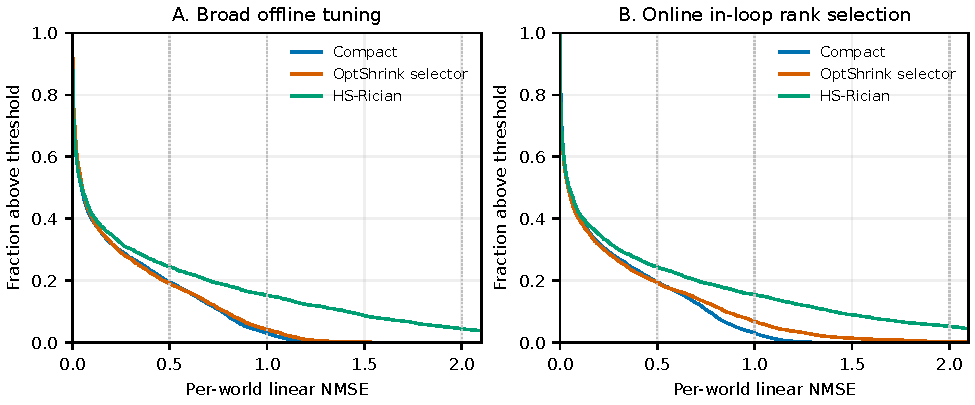
\includegraphics[width=\textwidth]{latest_distributions.pdf}
\caption{Primary empirical exceedance curves over the displayed threshold range, separately by study. Learned curves average the three model-specific empirical distributions on the same worlds; predictions are not independent channels. All values, including larger errors, are retained in the evidence arrays. A lower rate at one threshold does not imply a lower rate at every threshold.}
\end{figure*}
\begin{figure}[!t]
\centering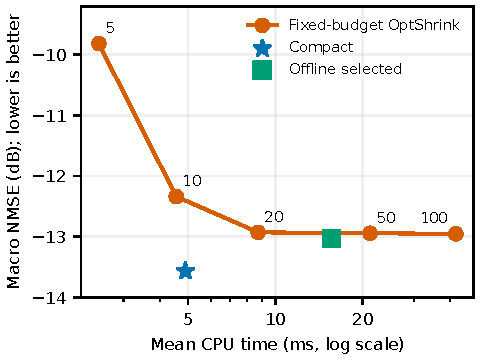
\includegraphics[width=\columnwidth]{latest_cost.pdf}
\caption{Study A accuracy--cost curve. Labels are fixed update budgets, each tuned separately for placement, rank and mixing. The selected lookup may use different budgets by noise/reference pair. No equal-runtime optimum is claimed.}
\end{figure}

\begin{table*}[!t]
\caption{Training-seed and test-bank summaries, kept distinct. Bank dB scores need not average to the score obtained after pooling their linear errors.}
\label{tab:broad-seeds}\centering\footnotesize
\setlength{\tabcolsep}{4pt}
\begin{tabular}{@{}llr@{}}\toprule
Study & Subset & NMSE (dB)\\
\midrule
A & Model 9101 & -13.676\\
A & Model 9102 & -13.327\\
A & Model 9103 & -13.692\\
A & Compact estimator (188 weights), bank 1 & -13.700\\
A & Compact estimator (188 weights), bank 2 & -13.559\\
A & Offline OptShrink, selected placement, bank 1 & -13.059\\
A & Offline OptShrink, selected placement, bank 2 & -13.064\\
B & Model 9101 & -13.759\\
B & Model 9102 & -13.417\\
B & Model 9103 & -13.765\\
B & Compact estimator (188 weights), bank 1 & -13.666\\
B & Compact estimator (188 weights), bank 2 & -13.648\\
B & Offline OptShrink, selected placement, bank 1 & -13.207\\
B & Offline OptShrink, selected placement, bank 2 & -13.183\\
B & Online rank + placement selection, bank 1 & -14.196\\
B & Online rank + placement selection, bank 2 & -14.050\\
B & Online rank, in-loop, bank 1 & -14.166\\
B & Online rank, in-loop, bank 2 & -14.149\\
\bottomrule
\end{tabular}
\end{table*}


\begin{table}[!t]
\caption{Study A: descriptive marginal averages over the other primary conditions. OptShrink is offline-selected. These are not additional independent tests.}
\label{tab:marginal-A}\centering\footnotesize
\setlength{\tabcolsep}{4pt}
\begin{tabular}{@{}llrrr@{}}\toprule
Study & Condition & Compact & OptShrink & Gain\\
\midrule
A & SNR -10 & -1.057 & -0.835 & 0.222\\
A & SNR -5 & -3.682 & -3.894 & -0.212\\
A & SNR 0 & -8.346 & -8.220 & 0.126\\
A & SNR 5 & -13.481 & -12.832 & 0.649\\
A & SNR 10 & -18.636 & -17.375 & 1.262\\
A & SNR 15 & -23.521 & -22.275 & 1.246\\
A & SNR 20 & -26.232 & -25.767 & 0.465\\
A & RSR 5 & -12.494 & -11.840 & 0.654\\
A & RSR 12 & -13.968 & -13.450 & 0.518\\
A & RSR 20 & -14.234 & -13.795 & 0.439\\
A & Paths 3--7 & -14.295 & -13.536 & 0.759\\
A & Paths 2 & -15.863 & -13.674 & 2.190\\
A & Paths 4 & -14.704 & -13.814 & 0.890\\
A & Paths 8 & -13.099 & -13.255 & -0.156\\
A & Paths 12 & -12.119 & -12.309 & -0.190\\
A & Paths 16 & -11.310 & -11.582 & -0.272\\
\bottomrule
\end{tabular}
\end{table}


\begin{table}[!t]
\caption{Study B: descriptive marginal averages over the other primary conditions. OptShrink is online in-loop rank selection. These are not additional independent tests.}
\label{tab:marginal-B}\centering\footnotesize
\setlength{\tabcolsep}{4pt}
\begin{tabular}{@{}llrrr@{}}\toprule
Study & Condition & Compact & OptShrink & Gain\\
\midrule
B & SNR -10 & -1.073 & -0.362 & 0.710\\
B & SNR -5 & -3.605 & -3.574 & 0.031\\
B & SNR 0 & -8.284 & -8.426 & -0.142\\
B & SNR 5 & -13.581 & -13.888 & -0.307\\
B & SNR 10 & -18.694 & -19.289 & -0.595\\
B & SNR 15 & -23.365 & -24.210 & -0.845\\
B & SNR 20 & -26.926 & -29.329 & -2.403\\
B & RSR 5 & -12.754 & -13.098 & -0.345\\
B & RSR 12 & -13.985 & -14.530 & -0.544\\
B & RSR 20 & -14.202 & -14.834 & -0.632\\
B & Paths 3--7 & -14.342 & -14.546 & -0.203\\
B & Paths 2 & -16.436 & -17.151 & -0.715\\
B & Paths 4 & -14.653 & -15.150 & -0.498\\
B & Paths 8 & -13.014 & -13.495 & -0.482\\
B & Paths 12 & -12.210 & -12.592 & -0.382\\
B & Paths 16 & -11.227 & -11.990 & -0.763\\
\bottomrule
\end{tabular}
\end{table}


\begin{table*}[!t]
\caption{Stress conditions, excluded from primary averages. Weak reference: SNR 5/RSR 0 dB. Nearly noiseless: SNR 60/RSR 12 dB. Both use random three-to-seven-path channels.}
\label{tab:broad-stress}\centering\footnotesize
\setlength{\tabcolsep}{4pt}
\begin{tabular}{@{}lllr@{}}\toprule
Study & Condition & Method & NMSE (dB)\\
\midrule
A & Weak reference & Compact estimator (188 weights) & -7.842\\
A & Weak reference & Offline OptShrink, selected placement & -11.905\\
A & Weak reference & EM-GS, 100 updates & -6.109\\
A & Nearly noiseless & Compact estimator (188 weights) & -6.693\\
A & Nearly noiseless & Offline OptShrink, selected placement & -66.886\\
A & Nearly noiseless & EM-GS, 100 updates & -65.604\\
B & Weak reference & Compact estimator (188 weights) & -7.787\\
B & Weak reference & Offline OptShrink, selected placement & -11.498\\
B & Weak reference & EM-GS, 100 updates & -6.261\\
B & Weak reference & Online rank + placement selection & -10.101\\
B & Weak reference & Online rank, in-loop & -10.101\\
B & Nearly noiseless & Compact estimator (188 weights) & -6.835\\
B & Nearly noiseless & Offline OptShrink, selected placement & -67.618\\
B & Nearly noiseless & EM-GS, 100 updates & -66.212\\
B & Nearly noiseless & Online rank + placement selection & -70.134\\
B & Nearly noiseless & Online rank, in-loop & -70.121\\
\bottomrule
\end{tabular}
\end{table*}


\subsection{Frozen Settings and Numerical Verification}

The online selector searches a shared rank, not separate ranks for each user. Its mixing strength and iteration count are inherited from the matching in-loop or final-only row in the offline lookup. Thus the rank comparison does not exhaust all possible classical policies. Candidate initialization uses only the first 21 pilots. After scoring the other nine, the winner starts again from all 30. Joint selection evaluates both placements and counts both searches in timing. Search work shared while generating several experimental arms is not used to understate standalone timing.

\begin{table*}[!t]
\caption{Broad offline settings. Within each placement, columns give rank, mixing factor and update count. The selected column chooses between those placements. Rank zero denotes no filtering.}
\label{tab:settings-broad}\centering\footnotesize
\setlength{\tabcolsep}{4pt}
\begin{tabular}{@{}lrrrrrrl@{}}\toprule
SNR / RSR & Loop $r$ & $\beta$ & $T$ & Final $r$ & $\beta$ & $T$ & Selected\\
\midrule
-10 / 5 & 1 & 0.75 & 5 & 2 & 1.0 & 50 & final\\
-10 / 12 & 1 & 0.5 & 5 & 1 & 0.75 & 5 & final\\
-10 / 20 & 1 & 0.75 & 5 & 1 & 0.75 & 5 & loop\\
-5 / 5 & 2 & 0.5 & 10 & 3 & 0.75 & 20 & final\\
-5 / 12 & 2 & 0.5 & 5 & 2 & 0.75 & 5 & loop\\
-5 / 20 & 3 & 0.75 & 5 & 3 & 0.75 & 5 & loop\\
0 / 5 & 4 & 0.5 & 20 & 5 & 0.75 & 100 & loop\\
0 / 12 & 4 & 0.5 & 10 & 5 & 0.75 & 10 & loop\\
0 / 20 & 4 & 0.5 & 10 & 7 & 1.0 & 5 & loop\\
5 / 5 & 7 & 0.5 & 100 & 8 & 1.0 & 100 & loop\\
5 / 12 & 7 & 0.5 & 20 & 8 & 1.0 & 20 & loop\\
5 / 20 & 8 & 0.75 & 10 & 8 & 1.0 & 10 & loop\\
10 / 5 & 9 & 1.0 & 100 & 9 & 0.75 & 100 & loop\\
10 / 12 & 10 & 0.75 & 20 & 9 & 1.0 & 50 & loop\\
10 / 20 & 10 & 1.0 & 20 & 10 & 1.0 & 20 & loop\\
15 / 5 & 9 & 0.5 & 50 & 10 & 1.0 & 100 & loop\\
15 / 12 & 10 & 0.75 & 50 & 10 & 1.0 & 50 & loop\\
15 / 20 & 10 & 0.75 & 50 & 10 & 1.0 & 50 & loop\\
20 / 5 & 11 & 1.0 & 100 & 13 & 1.0 & 100 & loop\\
20 / 12 & 12 & 1.0 & 50 & 12 & 1.0 & 50 & loop\\
20 / 20 & 11 & 0.75 & 50 & 11 & 1.0 & 50 & loop\\
\bottomrule
\end{tabular}
\end{table*}


Study A: all 4,096 test worlds regenerated exactly; 3,584 representative predictions replayed. Maximum recorded independent classical absolute output difference was $5.73\times10^{-13}$. An independent scalar-loop calculation reproduced every primary score. These checks test the saved implementation and data, not an external reproduction of the study.

Study B: all 4,096 test worlds regenerated exactly; 2,816 representative predictions replayed. Maximum recorded independent rank-selector absolute output difference was $1.26\times10^{-12}$. An independent scalar-loop calculation reproduced every primary score. These checks test the saved implementation and data, not an external reproduction of the study.

Study A also regenerated all 2,048 validation observations and replayed selection from saved scores. Study B independently checked both rank-score vectors, chosen settings and all-pilot refits with NumPy/SciPy. Its new audit did not independently replay HS-Rician again; that backend check is in Study A. Both studies passed finite-output, source-hash, checkpoint-hash and freeze-before-generation checks. No failed trial was removed. Full per-cell values and source records are supplied as JSON evidence in the manuscript archive; full observation and prediction arrays remain in the experimental archive.
